\documentclass[a4paper,11pt]{article}

\usepackage{latexsym}%symbole
\usepackage[empty]{fullpage}
\usepackage{titlesec}%alternatywne sekcje tytułowe
\usepackage{marvosym}%wiecej symboli
\usepackage[usenames,dvipsnames]{color}
\usepackage{verbatim}%wyświetlanie kodu
\usepackage{enumitem}%zmienianie layoutu
\usepackage[hidelinks]{hyperref}%?!?!?!
\usepackage{fancyhdr}%heders and footers
\usepackage[english]{babel}%znaki lokalne?
\usepackage{tabularx}% tabeli 
\usepackage{multicol}% wiele column
\usepackage{minted}% syntax hilighting
\input{glyphtounicode}

\usepackage{baskervillef}
\usepackage[T1]{fontenc}
%flow chatry
\usepackage{tikz}
\usetikzlibrary{shapes.geometric, arrows}
\usepackage{amssymb}
\usepackage{float}

\pagestyle{fancy}
\fancyhf{} 
\fancyfoot{}
\setlength{\footskip}{5pt}
\renewcommand{\headrulewidth}{0pt}
\renewcommand{\footrulewidth}{0pt}

\usepackage[bottom=0.5in,top=0.5in, left=0.5in ,right=0.5in]{geometry}

\urlstyle{same}

%\raggedbottom
\raggedright
\setlength{\tabcolsep}{0in}

\titleformat{\section}{
  \it\vspace{3pt}
}{}{0em}{}[\color{black}\titlerule\vspace{-5pt}]

\pdfgentounicode=1
%flowchatrts shapes

\definecolor{1}{RGB}{128, 147, 241}
\definecolor{2}{RGB}{114, 221, 247}
\definecolor{3}{RGB}{179, 136, 235}
\definecolor{4}{RGB}{247, 174, 248}

\tikzstyle{startstop} = [ellipse, rounded corners, minimum width=2cm, minimum height=1cm,text centered, draw=black,thick,fill=4]
\tikzstyle{io} = [trapezium,trapezium stretches=true,trapezium left angle=70,trapezium right angle=110,thick,minimum width=2cm,minimum height=0.85cm, text centered, draw=black,fill=1]
\tikzstyle{process} = [rectangle,minimum width=3cm,minimum height=0.85cm,text centered,text width=3cm,draw=black,thick,fill=2]
\tikzstyle{decision} = [diamond,minimum width=1cm, minimum height=1cm, text centered, draw=black, fill=3,thick]
\tikzstyle{arrow} = [thick,->,>=stealth]

\begin{document}
\begin{center}
    \begin{multicols}{2}
    \begin{flushleft}
    \large{Tymon Łazowy 2D nr.13} \\
    \end{flushleft}
    
    \begin{flushright}
    \large{04.04.2023}\\
    \end{flushright}
    \end{multicols}
    {\LARGE Sprawozdanie z informatyki nr 1} \\ \vspace{0pt}
\end{center}

\section{Treść zadanie}
\begin{center}
\large{Programownie część pierwsza}\\

\begin{itemize}[ label={}]
    \normalsize{\item{
    {1.0 - Wyświetl napis powitalny, 2 wiersze poniżej ndk, cls, pożegnanie}{} \\
    {1.1 - Wartość wyrażenia, 2 miejsca po przecinku: $\frac{2*3+17}{9}$ (wynik $2,56$) }{}\\
    {1.2 - Wartość wyrażenia, 3 miejsca po przecinku: $\frac{4^2+2*4*7+7^2}{5+37\div4}$ (wynik $8,491$) }{} \\
    {1.3 - Powitanie, cls, pole pow. i objętość sześcianu o boku 5,875 cm (2mpp) (p=207,09; obj=202,78) \\
    {1.4 - Pole objętość i suma długości krawędzi sześcianu o boku 7.225 cm (ze stałą)
$P=313,20; O=377,15; S=86,70$}{} \\
    {1.5 - Średnia arytmetyczna z 3 liczb - stałe( 7,12,16) oraz napis NDK
Średnia=11,67}{} \\
    {1.6 - Pole, objętość i suma długości krawędzi prostopadłościanu o bokach podanych
przez użytkownika (2mpp) }{} \\
    {1.7 - Pole, objętość i suma długości krawędzi walca o promieniu i wysokości podanych
przez użytkownika (pi jako stała)}{} \\
    {1.8 - Średnia arytmetyczna z 3 liczb podanych przez użytkownika z jego imieniem.}{} \\
    {1.9 - Pole prostokąta, ze sprawdzeniem danych (czy boki są większe od 0)}{} \\
    {1.10 - Czy dwie liczby podane przez użytkownika są podzielne przez siebie – pierwsza
przez drugą – uwaga na warunek podzielności}{} \\
    {1.11 - Równanie liniowe w pełnej postaci $(ax+b=c)$}{}\\
    {1.12 - Równanie $ax^2+bx+c=d$ kwadratowe lub liniowe – wyniki na dole ekranu}{}\\
    {1.13 - Wyświetlanie maksymalnej liczby z trzech podanych liczb całkowitych ze sprawdzeniem poprawności danych}{}\\
    {1.14 - Sprawdzenie możliwości skonstruowania trójkąta z trzech odcinków, których długości są losowymi liczbami rzeczywistymi, losowanymi z przedziału od <1,10> z jednym miejscem po przecinku (wyświetla liczby na górze i komunikat na dole ekranu}{}\\
}}}
\end{itemize}

\end{center}
%---------------------PROPONOWANE ROZWIĄZANIA-------------
%pagebreak 3, 6, 8, 9, 11
\section{Proponowane rozwiązania}
\subsection*{1.0}
%----------------1.0------------------
\begin{multicols}{2}
  \begin{flushleft}
    \begin{figure}[H]
    \centering  
\begin{tikzpicture}[node distance=1.5cm]

\node (start) [startstop] {Start};
\node (out1) [io, below of=start] {Wyświetl powitanie};
\node (out2) [io, below of=out1] {2 linie poniżej ndk};
\node (in1) [io, below of=out2] {poczekaj aż użytkownik ndk};
\node (pro1) [process, below of=in1] {Wyczyść terminal};
\node (out3) [io, below of=pro1] {Pożegnaj się};
\node (stop) [startstop, below of =out3]{stop};

\draw [arrow] (start) -- (out1);
\draw [arrow] (out1) -- (out2);
\draw [arrow] (out2) -- (in1);
\draw [arrow] (in1) -- (pro1);
\draw [arrow] (pro1) -- (out3);
\draw [arrow] (out3) -- (stop);

\end{tikzpicture}
    \caption{1.0 flowchart}
    \label{flow0}
\end{figure}
    \end{flushleft}
D: brak

W: brak
    \begin{flushright}
    \begin{minted}[framesep=1mm, baselinestretch=1.,linenos]{cpp}
    cout << "Witam w programie" << endl<< endl;
    cout << "Nacisnij dowolny kalwisz";
    getch();
    system("cls");
    cout << "do widzenia";
    getch();
\end{minted}
    \end{flushright}
\end{multicols}
\subsection*{1.1}
%-------1.1---------
\begin{multicols}{2}
  \begin{flushleft}
    \begin{figure}[H]
    \centering  
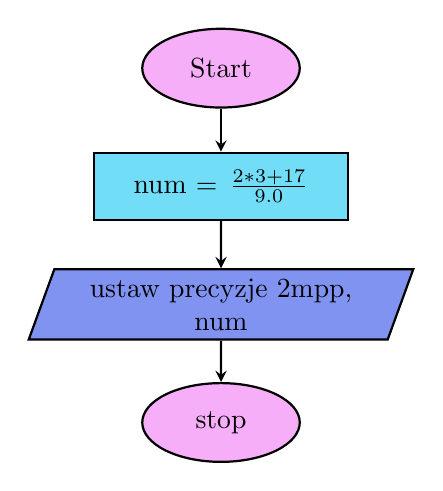
\begin{tikzpicture}[node distance=1.5cm]

\node (start) [startstop] {Start};
\node (out1) [process, below of=start] {num $=\frac{2*3+17}{9.0}$};
\node (out2) [io, below of=out1,text width=4.cm] {ustaw precyzje 2mpp,

num};
\node (stop) [startstop, below of =out2]{stop};

\draw [arrow] (start) -- (out1);
\draw [arrow] (out1) -- (out2);
\draw [arrow] (out2) -- (stop);

\end{tikzpicture}
    \caption{1.1 flowchart}
    \label{flow1}
\end{figure}
    \end{flushleft}
D:?

W: num Wartość wyrażenia $\in$ {2,56} 
    \begin{flushright}
    \begin{minted}[framesep=1mm, baselinestretch=1.,linenos]{cpp}
    double num = (2*3+17)/9.0;
    cout <<setprecision(3)<<num;
\end{minted}
    \end{flushright}
\end{multicols}
\subsection*{1.2}
%------------1.2------------
\begin{multicols}{2}
  \begin{flushleft}
    \begin{figure}[H]
    \centering  
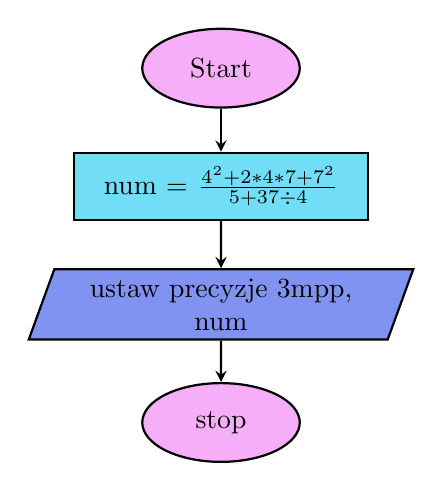
\begin{tikzpicture}[node distance=1.5cm]

\node (start) [startstop] {Start};
\node (out1) [process, below of=start,text width=3.5cm] {num $=\frac{4^2+2*4*7+7^2}{5+37\div4}$};
\node (out2) [io, below of=out1,text width=4.cm] {ustaw precyzje 3mpp,

num};
\node (stop) [startstop, below of =out2]{stop};

\draw [arrow] (start) -- (out1);
\draw [arrow] (out1) -- (out2);
\draw [arrow] (out2) -- (stop);

\end{tikzpicture}
    \caption{1.2 flowchart}
    \label{flow2}
\end{figure}
    \end{flushleft}
D:? 

W: num wartość wyrażenia $\in$ 8,491 
    \begin{flushright}
    \begin{minted}[framesep=1mm, baselinestretch=1.,linenos]{cpp}
float num = (pow(4,2)+2*4*7+pow(7,2))/(5+37/4.0);
cout <<setprecision(4)<<num;
\end{minted}
    \end{flushright}
\end{multicols}
\subsection*{1.3}
%--------------1.3-------------
\begin{multicols}{2}
  \begin{flushleft}
    \begin{figure}[H]
    \centering  
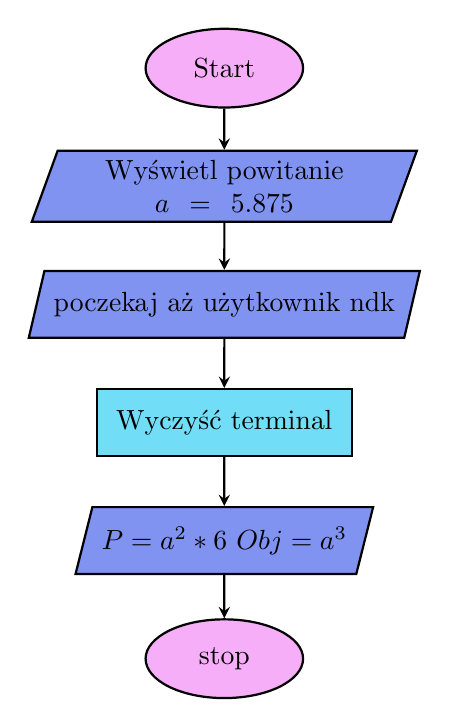
\begin{tikzpicture}[node distance=1.5cm]

\node (start) [startstop] {Start};
\node (out1) [io, below of=start,text width=4cm] {Wyświetl powitanie

$a=5.875$};
\node (in1) [io, below of=out1] {poczekaj aż użytkownik ndk};
\node (pro1) [process, below of=in1] {Wyczyść terminal};
\node (out2) [io, below of=pro1]{$P=a^2*6$ $Obj=a^3$};
\node (stop) [startstop, below of =out2]{stop};

\draw [arrow] (start) -- (out1);
\draw [arrow] (out1) -- (in1);
\draw [arrow] (in1) -- (pro1);
\draw [arrow] (pro1) -- (out2);
\draw [arrow] (out2) -- (stop);

\end{tikzpicture}
    \caption{1.3 flowchart}
    \label{flow3}
\end{figure}
    \end{flushleft}
D:a bok $\in$ {5.875} 

W: P,Obj wymiary $\in  \mathbb{R}$
    \begin{flushright}
    \begin{minted}[framesep=1mm, baselinestretch=1.,linenos]{cpp}
string pow ("witam w programie");
char* pow_arr = new char[pow.length()];
strcpy(pow_arr, pow.c_str());
for(n=0;n<=pow.length()n++){
    cout << pow_arr[n-1];
    Sleep(250);}
Sleep(2000);
system("cls");
float bok = 5.875;
float pole = 6.0*bok*bok;
float obj = 1.0*bok*bok*bok;
cout<<setprecision(3)<<"p="<<pole<<";obj="<< obj;
\end{minted}
    \end{flushright}
\end{multicols}

\pagebreak
\subsection*{1.4}
%--------------1.4-------------
\begin{multicols}{2}
  \begin{flushleft}
    \begin{figure}[H]
    \centering  
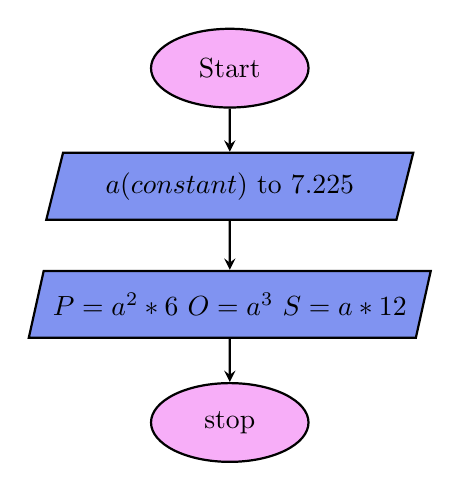
\begin{tikzpicture}[node distance=1.5cm]

\node (start) [startstop] {Start};
\node (out1) [io, below of=start,text width=4cm] {$a(constant)$ 
  to $ 7.225$};
\node (out2) [io, below of=out1]{$P=a^2*6$ $O=a^3$ $S= a*12 $};
\node (stop) [startstop, below of =out2]{stop};

\draw [arrow] (start) -- (out1);
\draw [arrow] (out1) -- (out2);
\draw [arrow] (out2) -- (stop);

\end{tikzpicture}
    \caption{1.4 flowchart}
    \label{flow4}
\end{figure}
    \end{flushleft}
 D: a bok $\in$ \{7.225\} 
 
 W: P,O,S wymiary $\in $ \{313,20; 377,15; 86,70\}
    \begin{flushright}
    \begin{minted}[framesep=1mm, baselinestretch=1.,linenos]{cpp}
cout <<fixed<< setprecision(2)<<\
"dla boku:"<<a << endl <<\
"P="<< a*a*6<< endl <<\
"O=" << a*a*a << endl<<\
"S="<< a*12;
\end{minted}
    \end{flushright}
\end{multicols}
\subsection*{1.5}
%--------------1.5-------------
\begin{multicols}{2}
  \begin{flushleft}
    \begin{figure}[H]
    \centering  
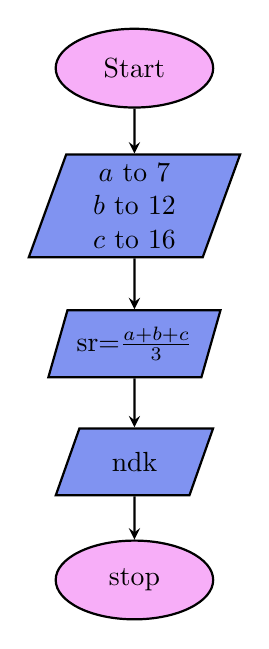
\begin{tikzpicture}[node distance=1.5cm]

\node (start) [startstop] {Start};
\node (out1) [io, below of=start,text width=1.5cm,yshift=-0.25cm] {$a$ to 7

$b$ to 12

$c$ to 16};
\node (in1) [io, below of=out1,yshift=-0.25cm] {sr=$\frac{a+b+c}{3}$};
\node (out2) [io, below of=in1]{ndk};
\node (stop) [startstop, below of =out2]{stop};

\draw [arrow] (start) -- (out1);
\draw [arrow] (out1) -- (in1);
\draw [arrow] (in1) -- (out2);
\draw [arrow] (out2) -- (stop);

\end{tikzpicture}
    \caption{1.5 flowchart}
    \label{flow5}
\end{figure}
    \end{flushleft}
 D: a,b,c parametry $\in$ \{7; 12; 16\}
 
 W: sr średnia parametrów $\in$ \{11,67\}
    \begin{flushright}
    \begin{minted}[framesep=1mm, baselinestretch=1.,linenos]{cpp}
double sr = (a+b+c)/3.0;
cout << fixed <<setprecision(2)<<\
"Srednia: " << sr << endl
\end{minted}
    \end{flushright}
\end{multicols}
\subsection*{1.6}
%--------------1.6-------------
\begin{multicols}{2}
  \begin{flushleft}
    \begin{figure}[H]
    \centering  
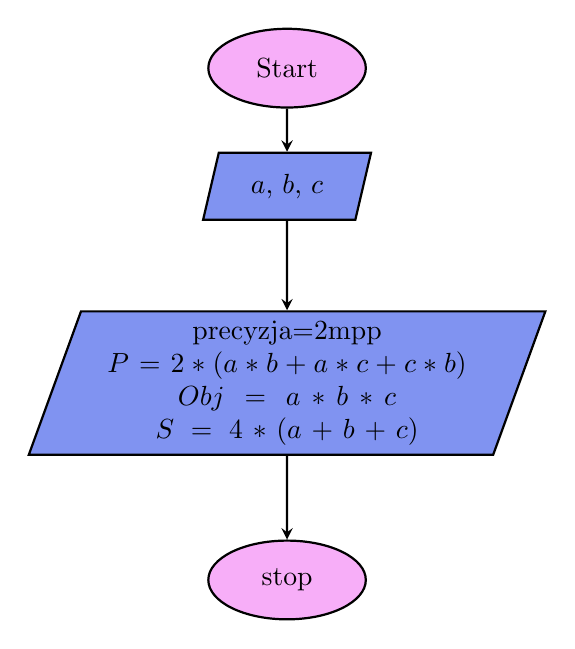
\begin{tikzpicture}[node distance=1.5cm]

\node (start) [startstop] {Start};
\node (in1) [io, below of=start,text width=1.5cm,yshift=0cm] {$a$, $b$, $c$};
\node (out1) [io, below of=in1,yshift=-1cm,text width=5cm] {precyzja=2mpp

$P=2*(a*b+a*c+c*b)$

$Obj=a*b*c$

$S=4*(a+b+c)$};
\node (stop) [startstop, below of =out1,yshift=-1cm]{stop};

\draw [arrow] (start) -- (in1);
\draw [arrow] (in1) -- (out1);
\draw [arrow] (out1) -- (stop);

\end{tikzpicture}
    \caption{1.6 flowchart}
    \label{flow6}
\end{figure}
    \end{flushleft}
 D: a,b,c parametry $\in$ $\mathbb{R}>0$
 
 W: P,Obj,S wymiary $\in$ $\mathbb{R}$
    \begin{flushright}
    \begin{minted}[framesep=1mm, baselinestretch=1.,linenos]{cpp}
float a;
float b;
float c;
cout<<"Prosze podac bok a:"; cin >> a;
cout <<"Prosze podac bok b:"; cin >> b;
cout <<"Prosze podac bok c:"; cin >> c;
cout<<fixed<<setprecision(2)<<\
"Objetosc jest równa="<<a*b*c<<endl<<\
"pole jest równe="<<2*(a*b+a*c+b*c)<<endl<<\
"Suma dlugosci krawedzi to="<<4*(a+b+c);
\end{minted}
    \end{flushright}
\end{multicols}

\pagebreak
\subsection*{1.7}
%--------------1.7-------------
\begin{multicols}{2}
  \begin{flushleft}
    \begin{figure}[H]
    \centering  
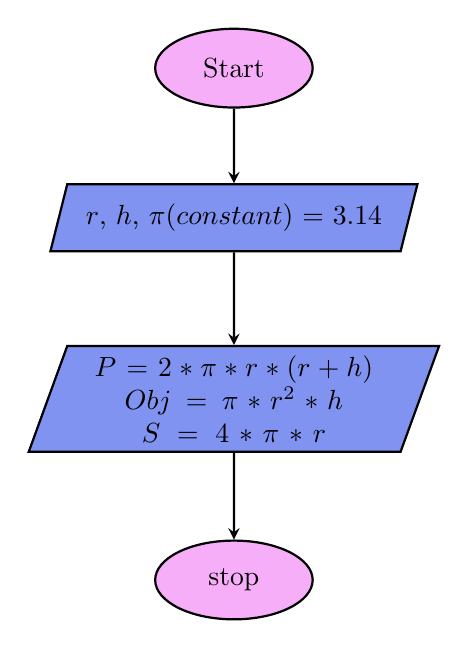
\begin{tikzpicture}[node distance=1.5cm]

\node (start) [startstop] {Start};
\node (in1) [io, below of=start,text width=4cm,yshift=-0.4cm] {$r$, $h$,
$\pi(constant)=3.14$};
\node (out1) [io, below of=in1,yshift=-.80cm,text width=4cm] {$P=2*\pi*r*(r+h)$

$Obj=\pi*r^2*h$

$S=4*\pi*r$};
\node (stop) [startstop, below of =out1,yshift=-0.80cm]{stop};

\draw [arrow] (start) -- (in1);
\draw [arrow] (in1) -- (out1);
\draw [arrow] (out1) -- (stop);


\end{tikzpicture}
    \caption{1.7 flowchart}
    \label{flow7}
\end{figure}
    \end{flushleft}
 D: r,h parametry $\in$ $\mathbb{R}>0$
 
 W: P,Obj,S wymiary $\in$ $\mathbb{R}$
    \begin{flushright}
    \begin{minted}[framesep=1mm, baselinestretch=1.,linenos]{cpp}
float r;
float h;
const float pi=3.14;
cout<<"Prosze podać promień:"; cin >> r;
cout <<"Prosze podac wysokosc:"; cin >> h;
cout<<fixed<<setprecision(2)<<\
"Objetosc jest równa="<<pi*r*r*h<<endl<<\
"pole jest równe="<<2*pi*r*(r+h)<<endl<<\
"Suma dlugosci krawedzi to="<<4*pi*r;
\end{minted}
    \end{flushright}
\end{multicols}
\subsection*{1.8}
%--------------1.8-------------
\begin{multicols}{2}
  \begin{flushleft}
    \begin{figure}[H]
    \centering  
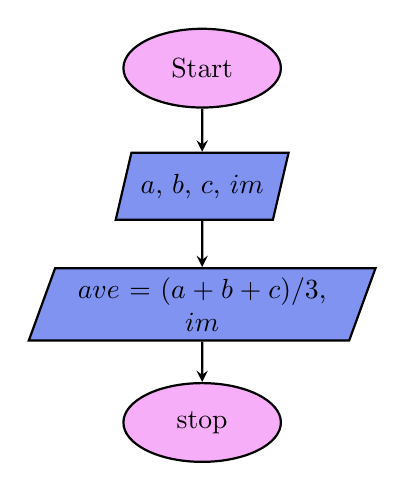
\begin{tikzpicture}[node distance=1.5cm]

\node (start) [startstop] {Start};
\node (in1) [io, below of=start,] {$a$, $b$, $c$, $im$ };
\node (out1) [io, below of=in1,text width=3.5cm] {$ave=(a+b+c)/3$, 

$im$};
\node (stop) [startstop, below of =out1]{stop};

\draw [arrow] (start) -- (in1);
\draw [arrow] (in1) -- (out1);
\draw [arrow] (out1) -- (stop);

\end{tikzpicture}
    \caption{1.8 flowchart}
    \label{flow8}
\end{figure}
    \end{flushleft}
 D: a, b, c, im; Liczy i imie użytkownika $\in$ $\mathbb{R}$
 
 W: ave średnia $\in$ $\mathbb{R}$
    \begin{flushright}
    \begin{minted}[framesep=1mm, baselinestretch=1.,linenos]{cpp}
float a;
float b;
float c;
string name;
cout<<"Podaj imię użytkownika:"; cin >> name;
cout<<"Prosze podać pierwszą liczbę:"; cin >> a;
cout<<"Prosze podać drugą liczbę:"; cin >> b;
cout<<"Prosze podać trzecią liczbę:"; cin >> c;
float ave = (a+b+c)/3;	
cout<<"średnia jest równa ="<<ave<<endl;
cout<<"Imie użytkownika to: "<<name<<endl;
\end{minted}
    \end{flushright}
\end{multicols}
\pagebreak
\subsection*{1.9}
%--------------1.9-------------
\begin{multicols}{2}
  \begin{flushright}
    
    \begin{figure}[H]
    \centering  
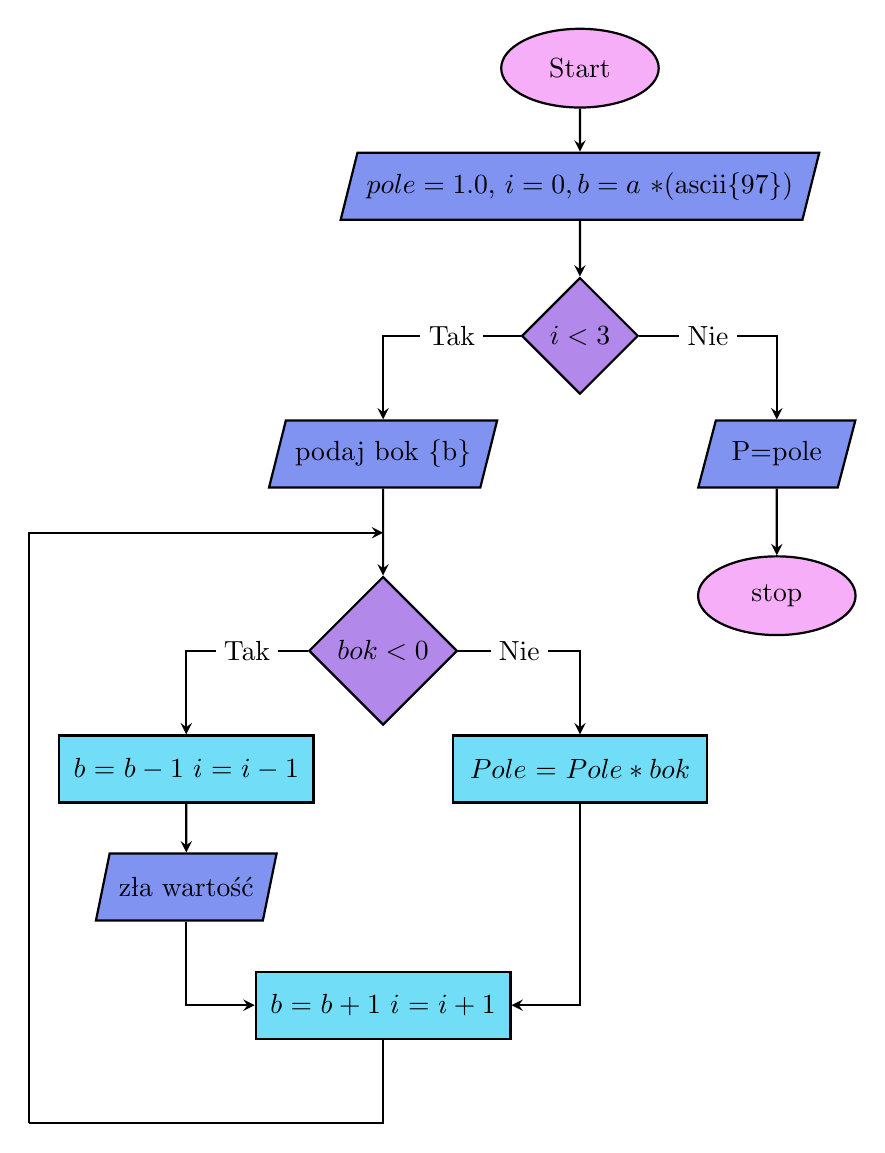
\begin{tikzpicture}[node distance=1.5cm]

\node (start) [startstop] {Start};
\node (in1) [io, below of=start,] {$pole=1.0$,  $i=0,b=a$  $\ast$(ascii\{97\})};
\node (dec1) [decision, below of=in1,yshift=-.4cm] {$i<3$};
\node (in2) [io, left of=dec1,yshift=-1.5cm,xshift=-1.cm] {podaj bok \{b\}};
\node (meet2)[coordinate,below of =in2,yshift=0.5cm]{};
\node (dec2) [decision, below of=meet2,] {$bok<0$};
\node (tak1) [process, left of=dec2,yshift=-1.5cm,xshift=-1.cm] {$b=b-1$ $i=i-1$};
\node (out1) [io, below of=tak1,] {zła wartość};
\node (nie1) [process, right of=dec2,yshift=-1.5cm,xshift=1.cm] {$Pole=Pole*bok$};
\node (pro2) [process, below of=dec2,yshift=-3cm] {$b=b+1$ $i=i+1$};
\node (out) [io, right of=dec1,yshift=-1.5cm,xshift=1.cm] {P=pole};
\node (stop) [startstop, below of=out,yshift=-0.3cm]{stop};
\node (meet)[coordinate,below of =pro2,xshift=-4.5cm]{};

\draw [arrow] (start) -- (in1);
\draw [arrow] (in1) -- (dec1);
\draw[arrow] (dec1) -| (out) node[pos=0.25,fill=white,inner sep=3]{Nie};
\draw [arrow] (out) -- (stop);
\draw[arrow] (dec1) -| (in2) node[pos=0.25,fill=white,inner sep=3]{Tak};
\draw [arrow] (in2) -- (dec2);
\draw[arrow] (dec2) -| (tak1) node[pos=0.25,fill=white,inner sep=3]{Tak};
\draw[arrow] (dec2) -| (nie1) node[pos=0.25,fill=white,inner sep=3]{Nie};
\draw [arrow] (tak1) -- (out1);
\draw [arrow] (out1) |- (pro2);
\draw [arrow] (nie1) |- (pro2);
\draw [thick] (pro2) |- (meet);
\draw [arrow] (meet) |- (meet2);
\end{tikzpicture}
    \caption{1.9 flowchart}
    \label{flow9}
\end{figure}
    \end{flushright}
    \begin{flushleft}
    \vspace{3cm} 
D: a,b,c parametry $\in$ $\mathbb{R}$
 
W: P pole $\in$ $\mathbb{R}$
 \end{flushleft}
    
    \begin{flushright}
     \vspace{7cm} 
    \begin{minted}[framesep=1mm, baselinestretch=1.,linenos]{cpp}
float bok()
{
	float input = 0;
	cout<<"prosze podać bok:"; cin>>input;
	if (input<=0 || cin.fail())
    {cout<<"podana wartość\
    jest nie poprawna";exit(1);}
	else {return input;}
}
int main()
{
	float a; float b;
	a=bok();
	b=bok();
	cout<<"pole jest równe: "<<a*b;
}
\end{minted}
    \end{flushright}
    \end{multicols}
    \pagebreak
\subsection*{1.10}
%--------------1.10-------------
\begin{multicols}{2}
\begin{flushleft}
\begin{figure}[H]
\centering  
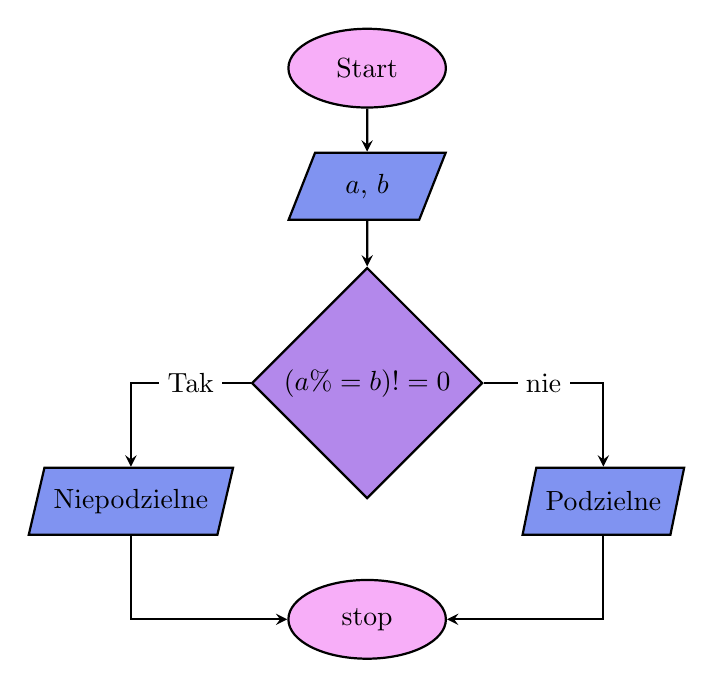
\begin{tikzpicture}[node distance=1.5cm]

\node (start) [startstop] {Start};
\node (in1) [io, below of=start,] {$a$, $b$};
\node (dec1) [decision, below of=in1,yshift=-1.cm] {$(a \%=b)!=0$};
\node (tak1) [io, left of=dec1, xshift=-1.5cm, yshift=-1.5cm] {Niepodzielne};
\node (nie1) [io, right of=dec1, xshift=1.5cm, yshift=-1.5cm] {Podzielne};
\node (stop)[startstop,below of=dec1,yshift=-1.5cm]{stop};

\draw [arrow] (start) -- (in1);
\draw [arrow] (in1) -- (dec1);
\draw[arrow] (dec1) -| (tak1) node[pos=0.25,fill=white,inner sep=3]{Tak};
\draw[arrow] (dec1) -| (nie1) node[pos=0.25,fill=white,inner sep=3]{nie};
\draw [arrow] (tak1) |- (stop);
\draw [arrow] (nie1) |- (stop);

\end{tikzpicture}
\caption{1.10 flowchart}
\label{flow10}
\end{figure}
\end{flushleft}
 D: a, b liczby$\in$ $\mathbb{R}$ czy są w rzeczywistym
 
 W: x podzielnść $\in$ prawda/fałsz
\begin{flushright}
\begin{minted}[framesep=1mm, baselinestretch=1.,linenos]{cpp}
int num1;
int num2;
cout<<"prosze podac pierwszą liczbe:"; cin >> num1;
cout<<"prosze podac drógą liczbe:"; cin >> num2;
num1 %= num2;
if(num1!=0){cout<<"liczny są niepodzielne"<< endl;
}else{cout<<"liczny są podzielne"<< endl;}
\end{minted}
\end{flushright}
\end{multicols}
\subsection*{1.11}
%--------------1.11-------------
\begin{multicols}{2}
\begin{flushleft}
\begin{figure}[H]
\centering  
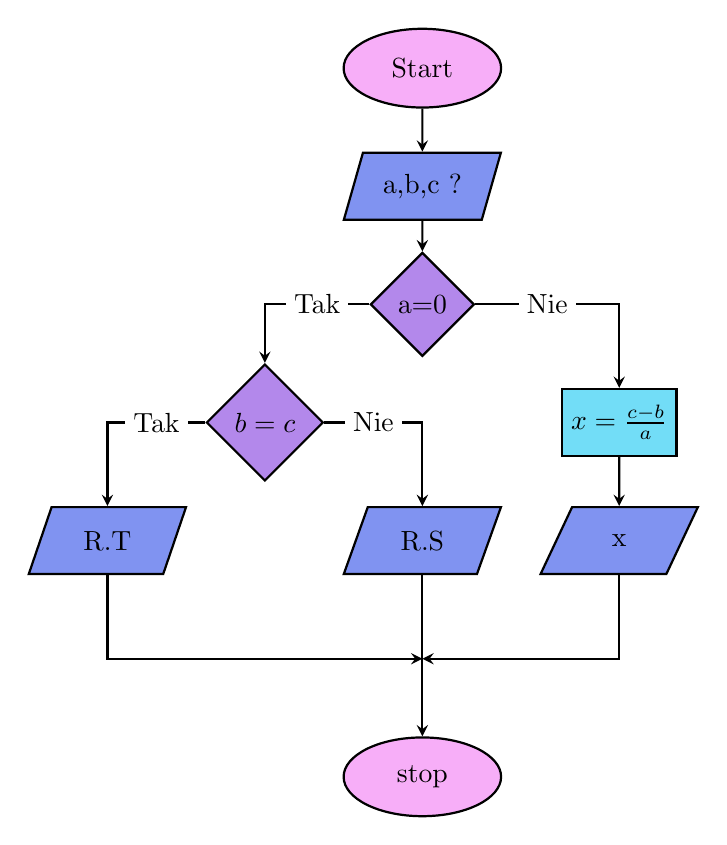
\begin{tikzpicture}[node distance=1.5cm]

\node (start) [startstop] {Start};
\node (in1) [io, below of=start] {a,b,c ?};
\node (dec1) [decision, below of=in1] {a=0};
\node (pro1) [rectangle,minimum height=0.85cm,text centered,draw=black,thick,fill=2, right of=dec1, xshift=1cm, yshift=-1.5cm] {$x=\frac{c-b}{a}$};
\node (in4) [io, below of =pro1]{x};
\node (dec2) [decision, left of=dec1, xshift=-0.50cm, yshift=-1.5cm] {$b=c$};
\node (in2) [io, right of=dec2, xshift=0.50cm, yshift=-1.5cm] {R.S};
\node (in3) [io, left of=dec2, xshift=-0.50cm, yshift=-1.5cm] {R.T};
\node (meeting)[coordinate,below of =in2]{};
\node (stop) [startstop, below of =meeting, yshift=0]{stop};

\draw [arrow] (start) -- (in1);
\draw [arrow] (in1) -- (dec1);
\draw[arrow] (dec1) -| (dec2) node[pos=0.25,fill=white,inner sep=3]{Tak};
\draw[arrow] (dec1) -| (pro1) node[pos=0.25,fill=white,inner sep=3]{Nie};
\draw[arrow] (dec2) -| (in3) node[pos=0.25,fill=white,inner sep=3]{Tak};
\draw[arrow] (dec2) -| (in2) node[pos=0.25,fill=white,inner sep=3]{Nie};
\draw [arrow] (pro1) -- (in4);   
\draw [arrow] (in4) |- (meeting);
\draw [thick] (in2) |- (meeting);
\draw [arrow] (in3) |- (meeting);
\draw [arrow] (meeting)--(stop);

\end{tikzpicture}
\caption{1.11 flowchart}
\label{flow11}
\end{figure}
\end{flushleft}
 Równanie: $ax+b=c$

D: a,b,c wyznaczniki $\in \mathbb R$

W: x rozwiązanie równania $\in \mathbb{R}$ 
 
\begin{flushright}
\begin{minted}[framesep=1mm, baselinestretch=1.,linenos]{cpp}
float a;
float b;
float c;
cout<<"prosze podać a:"; cin>>a;
cout<<"prosze podać b:"; cin>>b;
cout<<"prosze podać c:"; cin>>c;
if(a==0){
if(b==c){cout<<"Równanie tożsamośćowe"<<endl;}
else{cout<<"równanie sprzeczne"<< endl;}}
else{a=(c-b)/a;cout<<"x jest równy: "<< a<<endl;}
\end{minted}
\end{flushright}
\end{multicols}
\pagebreak
\subsection*{1.12}
%--------------1.12-------------
\begin{multicols}{2}
\begin{flushleft}
\begin{figure}[H]
\centering  
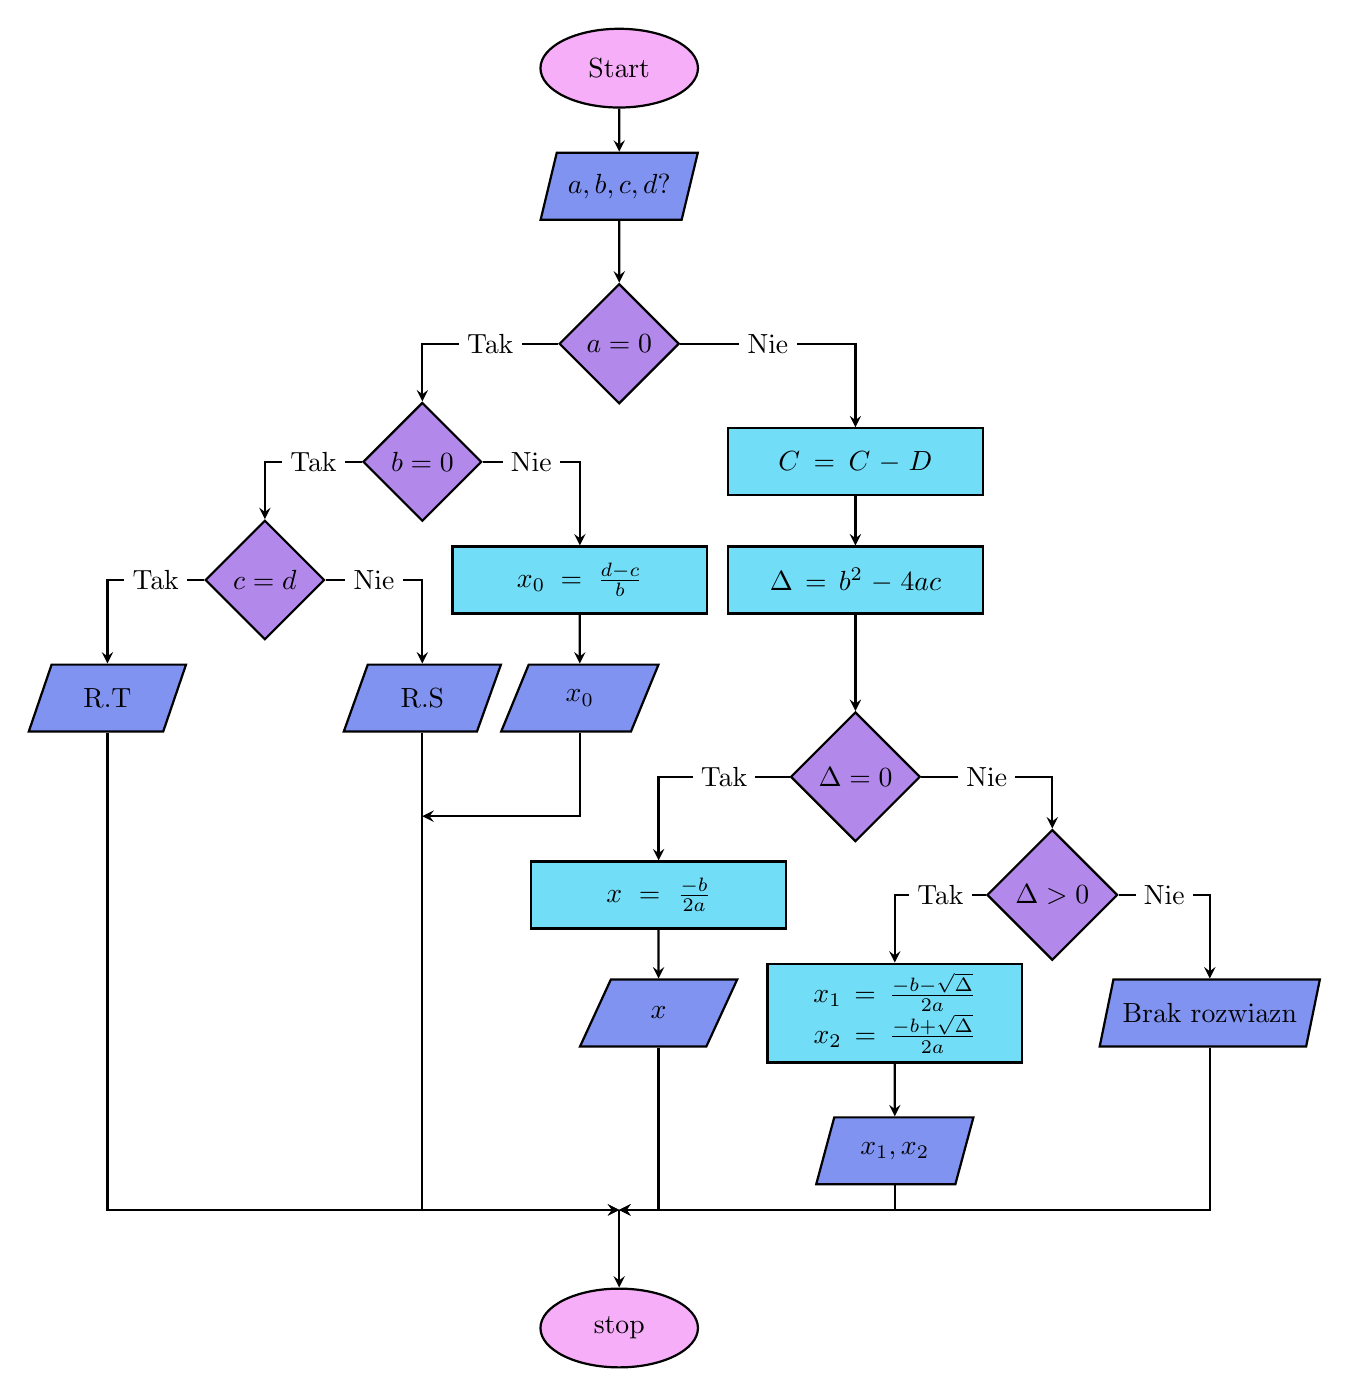
\begin{tikzpicture}[node distance=1.5cm]
\node (start) [startstop] {Start};
\node (in1) [io, below of=start] {$a,b,c,d ?$};

\node (dec) [decision, below of=in1,yshift=-0.5cm] {$a=0$};
%funkcja kwadratow
\node (nie) [process, right of=dec, xshift=1.5cm, yshift=-1.5cm] {$C=C-D$};
\node (pro2) [process, below of=nie] {$\Delta=b^2-4ac$};
\node (dec1) [decision, below of=pro2,yshift=-1.cm] {$\Delta=0$};
\node (tak1) [process, left of=dec1, xshift=-1.0cm, yshift=-1.5cm] {$x=\frac{-b}{2a}$};
\node (out1) [io, below of =tak1]{$x$};
\node (dec2) [decision, right of=dec1, xshift=1cm, yshift=-1.5cm] {$\Delta>0$};
\node (nie2) [io, right of=dec2, xshift=0.50cm, yshift=-1.5cm] {Brak rozwiazn};
\node (tak2) [process, left of=dec2, xshift=-0.50cm, yshift=-1.5cm] {$x_1=\frac{-b-\sqrt{\Delta}}{2a}$     $x_2=\frac{-b+\sqrt{\Delta}}{2a}$};
\node (out2) [io, below of =tak2,yshift=-0.25cm]{$x_1,x_2$};

\draw [arrow] (start) -- (in1);
\draw [arrow] (in1) -- (dec); 
\draw[arrow] (dec) -| (nie) node[pos=0.25,fill=white,inner sep=3]{Nie};
\draw [arrow] (nie) -- (pro2); 
\draw [arrow] (pro2) -- (dec1); 

\draw [arrow] (tak1) -- (out1);
\draw [arrow] (tak2) -- (out2);
\draw[arrow] (dec1) -| (dec2) node[pos=0.25,fill=white,inner sep=3]{Nie};
\draw[arrow] (dec1) -| (tak1) node[pos=0.25,fill=white,inner sep=3]{Tak};
\draw[arrow] (dec2) -| (tak2) node[pos=0.25,fill=white,inner sep=3]{Tak};
\draw[arrow] (dec2) -| (nie2) node[pos=0.25,fill=white,inner sep=3]{Nie};

%funkcja linowa
\node (1tak) [decision, left of =dec,xshift=-1.cm, yshift=-1.5cm]{$b=0$};
\node (2nie) [process, right of=1tak, xshift=0.5cm, yshift=-1.5cm] {$x_0=\frac{d-c}{b}$};
\node (1out) [io, below of =2nie]{$x_0$};
\node (2dec) [decision, left of=1tak, xshift=-0.50cm, yshift=-1.5cm] {$c=d$};
\node (3nie) [io, right of=2dec, xshift=0.50cm, yshift=-1.5cm] {R.S};
\node (3tak) [io, left of=2dec, xshift=-0.50cm, yshift=-1.5cm] {R.T};
\node (meeting)[coordinate,below of =start,yshift=-13cm]{};
\node (stop) [startstop, below of =meeting, yshift=0]{stop};
\node (mid)[coordinate,below of =3nie]{};

\draw[arrow] (dec) -| (1tak) node[pos=0.25,fill=white,inner sep=3]{Tak};
\draw[arrow] (1tak) -| (2dec) node[pos=0.25,fill=white,inner sep=3]{Tak};
\draw[arrow] (1tak) -| (2nie) node[pos=0.25,fill=white,inner sep=3]{Nie};
\draw[arrow] (2dec) -| (3tak) node[pos=0.25,fill=white,inner sep=3]{Tak};
\draw[arrow] (2dec) -| (3nie) node[pos=0.25,fill=white,inner sep=3]{Nie};
\draw [arrow] (2nie) -- (1out);
\draw [arrow] (3nie) |- (meeting);
\draw [arrow] (3tak) |- (meeting);
\draw [arrow] (1out) |- (mid);
\draw [arrow] (nie2) |- (meeting);
\draw [arrow] (out2) |- (meeting);
\draw [arrow] (out1) |- (meeting); 
\draw [arrow] (meeting)--(stop);
\end{tikzpicture}
\caption{1.12 flowchart}
\label{flow12}
\end{figure}
\end{flushleft}
Równanie: $ax^2+bx+c=d$

D: a,b,c,d wyznaczniki $\in \mathbb R$ 

W: $x, x_0,x_1,x_2$ rozwiązanie równania $\in \mathbb{R}$  
\end{multicols}
\begin{flushright}
\begin{minted}[framesep=1mm, baselinestretch=1.,linenos]{cpp}
float a; cout<<"prosze podać a:"; cin>>a; float b; cout<<"prosze podać b:"; cin>>b;
float c; cout<<"prosze podać c:"; cin>>c; float d; cout<<"prosze podać d:"; cin>>d;
float delta; gotoxy(0,25);
if(a==0){
	if(b==0){
		if(c==d){cout<<"Równanie tożsamośćowe"<<endl;}
		else{cout<<"równanie sprzeczne"<< endl;}}
	else{b=(d-c)/b;cout<<"x jest równy: "<<b<<endl;}
}else{  c=c-d;
        float delta=pow(b,2)-(4.0*a*c);
	if(delta==0){a=((-b)/(2*a));cout<<"x jest równy: "<< a <<endl;
	}else{
		if(delta>0){cout<<"x1 jest równy: "<< ((-b-sqrt(delta))/(2*a))<<endl;
			cout<<"x2 jest równy: "<<((-b+sqrt(delta))/(2*a))<<endl;
		}else{cout<<"brak rozwiązń"<<endl;}}}
\end{minted}
\end{flushright}

\subsection*{1.13}
%--------------1.13-------------
\begin{multicols}{2}
\begin{flushleft}
\begin{figure}[H]
\centering  
\begin{tikzpicture}[node distance=1.5cm]

\node (start) [startstop] {Start};
\node (in1) [io, below of=start,text width=2.5cm, yshift=-0.2cm] {arr=\{a,b,c\} ?

i=0, n=0};
\node (dec1) [decision, below of=in1, yshift=-1.5cm] {n<=3};
\node (tak1) [io, left of=dec1, xshift=-1cm, yshift=-1.5cm] {max = arr[i]};
\node (stop) [startstop, below of =tak1,yshift=-0.5cm]{stop};
\node (nie1) [decision, right of=dec1, xshift=0.50cm, yshift=-2.5cm] {arr[n]>arr[i]};
\node (tak2) [rectangle,minimum height=0.85cm,text centered,draw=black,thick,fill=2,left of=nie1,xshift=-1.2cm, yshift=-0.8cm] {i=n};
\node (nie2) [coordinate, right of=nie1,xshift=1.cm,yshift=0cm]{};

\node (meet) [coordinate, below of=in1,yshift=0.2cm]{};
\node (meet2) [coordinate, right of=pro2,xshift=0.2cm,yshift=-1cm]{};
\node (meet3) [coordinate, below of=nie1,yshift=0cm]{};
\node (pro2) [rectangle,minimum height=0.85cm,text centered,draw=black,thick,below of=meet3, yshift=0cm,fill=2] {n+1};

\draw [arrow] (start) -- (in1);
\draw [arrow] (in1) -- (dec1);
\draw[arrow] (dec1) -| (tak1) node[pos=0.25,fill=white,inner sep=3]{Tak};
\draw[arrow] (dec1) -| (nie1) node[pos=0.25,fill=white,inner sep=3]{Nie};
\draw[arrow] (nie1) -| (tak2) node[pos=0.25,fill=white,inner sep=3]{Tak};
\draw[thick] (nie1) -| (nie2) node[pos=0.25,fill=white,inner sep=3]{Nie};   
\draw [arrow] (nie2) |- (meet3);
\draw [arrow] (tak2) |- (meet3);
\draw [arrow] (meet3) -- (pro2);
\draw [thick] (pro2) -| (meet2);
\draw [arrow] (meet2) |- (meet);
\draw [arrow] (tak1)--(stop);

\end{tikzpicture}
\caption{1.13 flowchart}
\label{flow13}
\end{figure}
\end{flushleft}
D: a,b,c liczby $\in \mathbb{N}_0$

W: max najwieksza liczba $\in \mathbb{N}_0$ 
\begin{flushright}
\begin{minted}[framesep=1mm, baselinestretch=1.,linenos]{cpp}
int n = 3;
int t;
int arr[n];
int i=0;
while(i<n)
{   cout << "prosze podać "<< i+1 <<" liczbe:";
    cin >> t;
    arr[i]={t};
    i++;}
n = 0;
i = 0;
while(n<sizeof(arr)/sizeof(arr[0]))
{	if(arr[n]>arr[i]){i=n;}
    n++;}	
cout << "max number is: " << arr[i];
\end{minted}
\end{flushright}
\end{multicols}
\subsection*{1.14}
%--------------1.14-------------
\begin{multicols}{2}
\begin{flushleft}
\begin{figure}[H]
\centering  
\begin{tikzpicture}[node distance=1.5cm]

\node (start) [startstop] {Start};
\node (pro1) [process, below of=start,text width=2.5cm, yshift=-0.2cm,text width=4cm,] {zaok.dół(a,b,c random $\in \mathbb{R}$<0,1>*100)/10 };
\node (pro2) [process, below of=pro1,text width=2.5cm, yshift=-0.2cm] {posortuj a,b,c rosnąco};
\node (dec1) [decision, below of=pro2, yshift=-1.cm] {a+b>c};
\node (tak1) [io, left of=dec1, xshift=-0.8cm, yshift=-1.5cm] {można trójkąt};
\node (nie1) [io, right of=dec1, xshift=0.8cm, yshift=-1.5cm] {nie można};
\node (meet) [coordinate,below of =dec1,yshift=-1cm]{};
\node (stop) [startstop, below of =meet]{stop};


\draw [arrow] (start) -- (pro1);
\draw [arrow] (pro1) -- (pro2);
\draw [arrow] (pro2) -- (dec1);
\draw[arrow] (dec1) -| (tak1) node[pos=0.25,fill=white,inner sep=3]{Tak};
\draw[arrow] (dec1) -| (nie1) node[pos=0.25,fill=white,inner sep=3]{Nie};   
\draw [arrow] (tak1)|-(meet);
\draw [arrow] (nie1)|-(meet);
\draw [arrow] (meet)--(stop);

\end{tikzpicture}
\caption{1.14 flowchart}
\label{flow14}
\end{figure}
\end{flushleft}
D: brak

W: możliwość zbudownia trójkąta \{tak, nie\}
\begin{flushright}
\begin{minted}[framesep=1mm, baselinestretch=1.,linenos]{cpp}
int n = 3;
float a[n];
float b;

for(int i=0;i<n;i++)
{a[i-1]={ceil((rand()/ double(RAND_MAX))*100)/10+1};}

for(int i=0;i<n;i++)
{for(int j=0;j<n;j++)
{if(a[i-1]<a[j-1])
{b=a[i-1];a[i-1]=a[j-1];a[j-1]=b;}}}
	
gotoxy(0,0);
print_arr(a,n);
gotoxy(0,28);
if(a[-1]+a[0]>a[1]){cout<<"tak"<<endl;}
else{cout<<"nie"<<endl;}
\end{minted}
\end{flushright}
\end{multicols}
\subsection*{1.15}
%--------------1.15-------------

\begin{minted}[framesep=1mm, baselinestretch=1.,linenos]{cpp}
	srand(time(NULL));
	int num1;
	int num2;
	int opcja;
	float wynik;
	cout<<"podaj liczbe: ";cin>>num1;
	cout<<"podaj liczbe: ";cin>>num2;
	int los1=num1+rand()%(num2-num1+1);
	int los2=num1+rand()%(num2-num1+1);
	
	gotoxy(0,20);
	cout<<"1:"<<los1<<" 2: "<<los2;
	gotoxy(40,3);
	cout<<"menu:"<<endl<<\
	"1: dodawanie"<<endl<<\
	"2: odejmowanie"<<endl<<\
	"3: mnożenie"<<endl<<\
	"4: dzielenie"<<endl<<\
	"5: dzielnie całkowite"<<endl<<\
	"6: reszta z dzieleni"<<endl<<\
	"7: pierwiastek kwadratowy z 2x-4y^2 "<<endl;
	
	cout<<"opcja:"; cin>>opcja;
	
	if(opcja==1){wynik=los1+los2;}
	else if(opcja==2){wynik=los1-los2;}
	else if(opcja==3){wynik=los1*los2;}
	else if(opcja==4&&los2!=0){wynik=round((los1/1.0)/los2*100)/100;}
	else if(opcja==5&&los2!=0){wynik=los1/los2;}
	else if(opcja==6&&los2!=0){wynik=los1%los2;}
	else if(opcja==7&&(2*num1-4*num2*num2)>0)
    {wynik=sqrt(2*num1-4*num2*num2);wynik=round(wynik*100)/100;}
	else{cout<<"dla tych liczb nie ma wyniku"<<endl;}
	gotoxy(0,22);
	cout<<"wynik jest równy:"<<wynik<<endl; 
	cout<<"NDK";
	getch();
\end{minted}
\pagebreak

%-------------alternatywne rozwiązamnia
\section{Alternatywne rozwiązania}
\begin{center}
\large \textbf{python}
\end{center}
\begin{multicols}{2}
\begin{flushleft}
\subsection*{1.0}
\begin{minted}[framesep=1mm, baselinestretch=1.,linenos]{python}
print("Witaj w programie\n\n\n")
print("Naciśnij dowolny klawisz")
m.getch()
os.system("cls")
print("Do widzenia")
m.getch()
\end{minted}

\subsection*{1.1}

\begin{minted}[framesep=1mm, baselinestretch=1.,linenos]{python}
print(round((2*3+17)/9,2))
m.getch()
\end{minted}

\subsection*{1.2}

\begin{minted}[framesep=1mm, baselinestretch=1.,linenos]{python}
print(round((4**2+2*4*7+7**2)/(5+37/4),3))
\end{minted}

\subsection*{1.3}

\begin{minted}[framesep=1mm, baselinestretch=1.,linenos]{python}
print("Witaj w programie\n\n\n")
print("Naciśnij dowolny klawisz")
m.getch()
os.system("cls")

bok=5.875
print(\
"pole pow:", round(bok**2*6,2) ,\
"obj:", round(bok**3,2))
\end{minted}

\subsection*{1.4}
\begin{minted}[framesep=1mm, baselinestretch=1.,linenos]{python}
bok=7.225
print(\
"pole pow:", round(bok**2*6,2) ,\
"\nobj:", round(bok**3,2),\
"\nsuma krawedzi:",round(bok*12,2))
\end{minted}

\subsection*{1.5}
\begin{minted}[framesep=1mm, baselinestretch=1.,linenos]{python}
a=7
b=12
c=16

print("naciśnij dowolny klawisz")
m.getch()
print("średnia:",round((7+12+16)/3,2))
\end{minted}

\begin{minipage}{3cm}
\subsection*{1.6}
\begin{minted}[framesep=1mm, baselinestretch=1.,linenos]{python}
a = float(input("Prosze podac bok a:"))
b = float(input("Prosze podac bok b:"))
c = float(input("Prosze podac bok c:"))
print(\
"obj:", round(a*b*c,2),\
"\npole pow:", round(2*(a*b+a*c+b*c),2) ,\
"\nsuma krawedzi:",round(4*(a+b+c),2))
\end{minted}
\end{minipage}
\end{flushleft}
\begin{flushright}
\subsection*{1.7}
\begin{minted}[framesep=1mm, baselinestretch=1.,linenos]{python}
r = float(input("Prosze podac bok r:"))
h = float(input("Prosze podac bok h:"))
pi = float(3.14)
print(\
"obj:", round(pi*r*r*h,2),\
"\npole pow:", round(2*pi*r*(r+h),2) ,\
"\nsuma krawedzi:",round(4*pi*r,2))
\end{minted}

\subsection*{1.8}

\begin{minted}[framesep=1mm, baselinestretch=1.,linenos]{python}
name = input("Prosze podac imie użytkownika:")
a = float(input("Prosze podac liczbe a:"))
b = float(input("Prosze podac liczbe b:"))
c = float(input("Prosze podac liczbe c:"))
print("średnia:", (a+b+c)/3,"\nimię :",name)
\end{minted}

\subsection*{1.9}
\begin{minted}[framesep=1mm, baselinestretch=1.,linenos]{python}
bok=1.0
pole=1.0
i=0
while i < 3:
    try:
        bok = float(input("Prosze podac bok: "))
    except ValueError:
        print("podana wartosc jest niepoprawna\n")
        continue
    if bok < 0:
        
        print("podana wartosc jest niepoprawna\n")
    else:
        pole=pole*bok
        i += 1
print("pole prostokat to:",pole)
\end{minted}
\subsection*{1.10}
\begin{minted}[framesep=1mm, baselinestretch=1.,linenos]{python}
num1 = int(input("Prosze pierwszą liczbe: "))
num2 = int(input("Prosze pierwszą liczbe: "))
num1 %= num2 
if num1 == 0:print("podzielne")
else:print("nie podzielne")
\end{minted}
\end{flushright}
\pagebreak
\subsection*{1.11}
\begin{minted}[framesep=1mm, baselinestretch=1.,linenos]{python}
a = float(input("Prosze podać a: "))
b = float(input("Prosze podać b: "))
c = float(input("Prosze podać c: ")) 

if a == 0:
    if b==c:print("Równanie tożsamośćowe") 
    else:print("Równanie sprzeczne")    
else:print("x jest równy:", (c-b)/a)
\end{minted}
\subsection*{1.12}
\begin{minipage}{3cm}
\begin{minted}[framesep=1mm, baselinestretch=1.,linenos]{python}
a = float(input("Prosze podać a: "))
b = float(input("Prosze podać b: "))
c = float(input("Prosze podać c: "))
d = float(input("Prosze podać d: ")) 
if a == 0:
    if b==0:
        if c==d:print("Równanie tożsamośćowe") 
        else:print("Równanie sprzeczne")    
    else:print("x jest równy:", (d-c)/b)
else:
    c=c-d
    delta = b**2-(4*a*c)
    print("delta:", delta)
    if delta==0: print("x jest równy:", (-b)/(2*a))
    else:
        if delta>0:
            print("x1 jest równy:", (-b-mm.sqrt(delta))/(2*a))
            print("x2 jest równy:", (-b+mm.sqrt(delta))/(2*a))
        else: print("brak rozwiązań")
\end{minted}
\end{minipage}
\subsection*{1.13}
\begin{minted}[framesep=1mm, baselinestretch=1.,linenos]{python}
temp={}
i=0
while i < 3:
    try:
        num1 = int(input("Prosze podac liczbe: "))
    except ValueError:
        print("podana wartosc jest niepoprawna")
        continue
    temp[i] = num1
    i=i+1
i=0
while i<3:
    if temp[0]<temp[i]:temp[0]=temp[i]
    i=i+1

print("Maksymalna liczba to:",temp[0])
\end{minted}
\vspace{3cm}
\end{multicols}
\subsection*{1.14}
\begin{minipage}{3cm}
\begin{minted}[framesep=1mm, baselinestretch=1.,linenos]{python}
temp={}
i=0
while i < 3:
    temp[i]=secrets.randbelow(90)/10+1
    i=i+1
print(temp)
i=0
while i<3:
    if temp[i]>=sum(temp.values())-temp[i]:i=4
    i=i+1
if i>=4:print("\n\n\n\n\n\n\n\n\n\n\n\n\n\n\n\n\n\n\n\n\n\n\nnie można")
else:print("\n\n\n\n\n\n\n\n\n\n\n\n\n\n\n\n\n\n\n\n\n\nmożna")
\end{minted}
\end{minipage}


%--------------Programy użyte----------
\section{Programy użyte do wykonoania zadań}  
\LaTeX, google chrome, overleaf, dev c++, python, visual studio code, notepad++, git, github, Sumatra PDF, Total comander  
\section{Wnioski i uwagi} 
\begin{center}
 \large{Zadanie mi się bardzo podobało i nie mam żadnych uwag.}   
\end{center}
 
\end{document}
